\documentclass[version=last,fontsize=13pt]{scrartcl}


\usepackage{pdfpages}
\usepackage{graphicx}
\usepackage{indentfirst}

\usepackage{titlesec}
\usepackage{caption}

\titlespacing*{\section}{0pt}{3ex}{3ex}
\titlespacing*{\subsection}{0pt}{1.5ex}{1.5ex}
\titlespacing*{\subsubsection}{0pt}{1.5ex}{1.5ex}

\usepackage[margin = 0.8in]{geometry}

%my own paragraph for which the text that follows starts on a new line
\newcommand{\myparagraph}[1]{\paragraph{#1}\mbox{}\\}

% dont number sections
\setcounter{secnumdepth}{0}

\usepackage{wrapfig}
\usepackage{float}

\usepackage{caption}
\usepackage{subcaption}

\usepackage{tabularx}
\begin{document}

\begin{titlepage}
	\begin{center}	
		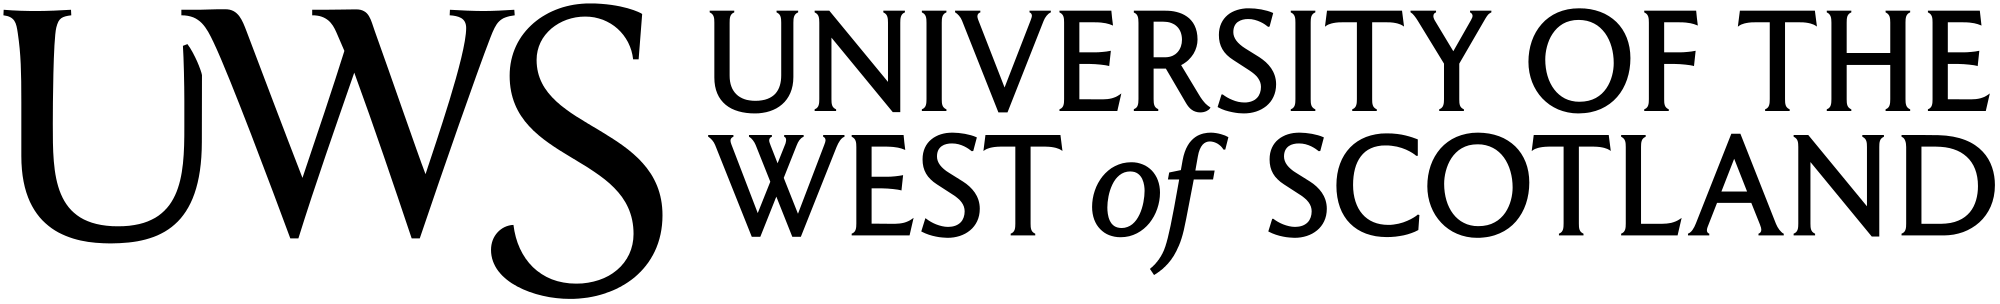
\includegraphics[width = 5cm,height = 1.5cm]{./imgs/uws_logo.png}\\[5cm]
	
	 { \huge \bfseries %
		How can Android Packed malware be detected and prevented?\\} 

	\vspace{6cm}			
			
		\begin{flushright}
				\large Student:\\
				Marius-Lucian Olariu\\[1cm]
		\end{flushright}
		
	
		\begin{flushleft}
			 \large
				Supervisor: \\
				Dr. Zeeshan Pervez \\[1cm]
		\end{flushleft}
		
	\vspace{2cm}	
	
		
		\vfill

			{\large {Paisley \\ 2019}}
		\end{center}
\end{titlepage}

\renewcommand{\labelenumi}{\roman{enumi}}

\newpage

\tableofcontents

\newpage

\listoffigures

\listoftables

\newpage


\section{Introduction}(5p - 500w)\\


%add information from the presentation slides and speakers notes

%summarise the traditional packaging technique
	Android is an \textbf{O}perating \textbf{S}ystem (OS) designed for mobile devices like tablets and smartphones and is currently the market leader  of mobile operating systems since of 2016 (Mobile OS Market Share 2018, 2019). Android has been the leading mobile OS in phones sold since 2011 as can be seen in Figure~\ref{aStats} (Mobile OS Market Share 2018, 2019). The CEO of Google, Sundar Pichai, declared at Google I/O 2017 that there are over two billion smartphones running Android OS  (Google I/O 2017, n.d). The success of Android is due to the fact that is very efficient (uses a modified version of the Linux kernel) and open-source.  The fact that Android is open-source and the large number of users it has attracts a lot of attackers to develop malware (huge material gains and prestige). The problem of Android malware is similar to the one Windows OS faces, in other words, because most of the personal computers run Windows most of the  malware targets Windows systems and not Linux or macOS systems. Another fact that makes Android so appealing to malware authors is the fact that is very easy to install applications from unknown sources and  there are many third-party markets for distribution of  Android applications.\\ 

	\begin{figure}[H]

		\caption{Global market share sales by mobile OSs from 2009 to 2018}
		\label{aStats}

		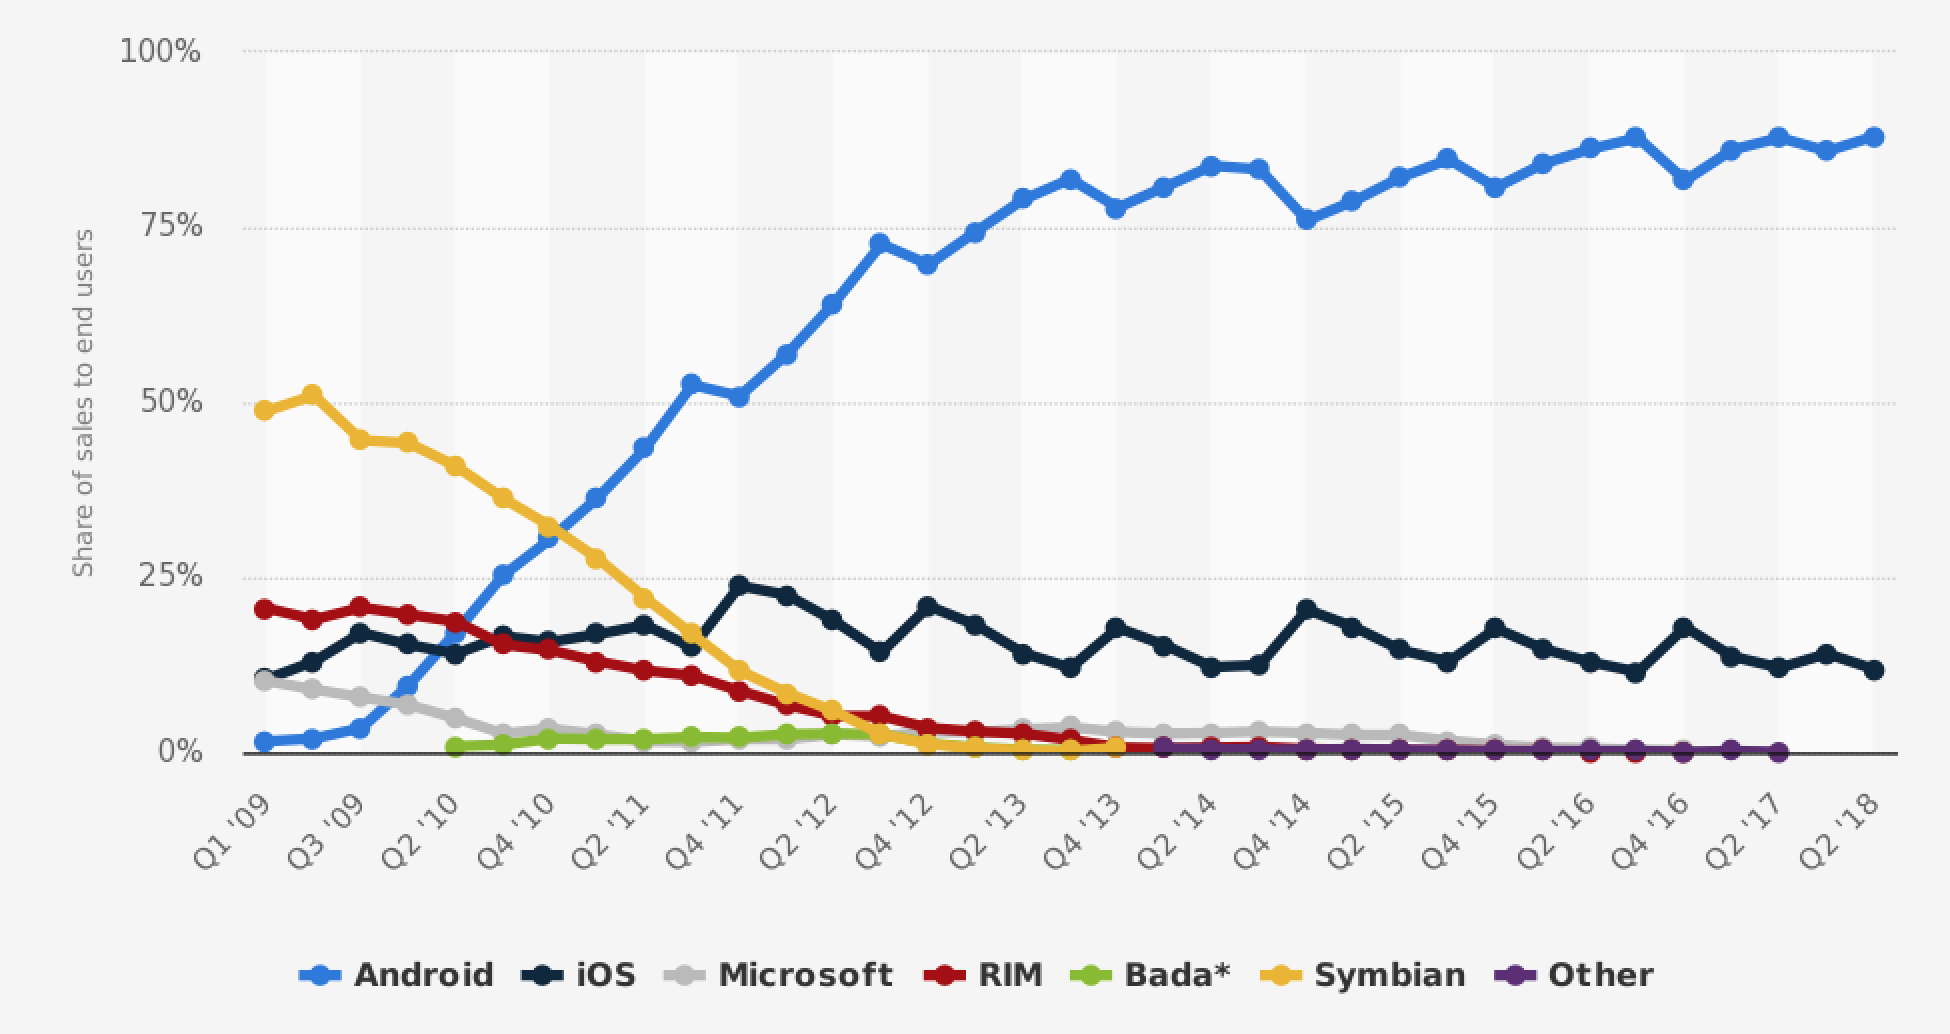
\includegraphics[scale = 0.48]{./imgs/androidStats.png}
	\end{figure}
	
	\indent
	Android applications are distributed and installed using the \textbf{A}ndroid \textbf{P}ac\textbf{k}age (.apk) format. The apk format is essentially an archive (was extended from JAR and ZIP) that contains the application compiled code, resources, certificates and the manifest file. Because an apk file it is just an archive it can be easily unarchived, thus it a fairly straight process to get to the complied code of a certain application once you have the apk file. For Android the compiled code is in \textbf{D}alvik \textbf{Ex}ecutable (DEX) format and because executable code is hard to understand for a human it needs to be further converted. DEX files can be converted to a human-readable format known as \textit{smali} using open-source tools like \textit{Apktool} (Tumbleson, n.d.). Moreover, \textit{Apktool} recovers the xml files and Android manifest file to a form close to the orignal ones. Typically, a smali file coresponds to a Java class code. In order to add malicious code the attacker can add smali code in the app files or add new smali files containg malicious code. For instance one could write a broadcast receiver that reads and sends the phone contacts of the users to a webserver and is triggered when the user restarts his phone, this does not need too much effort from an attacker. Once the malicious code is added to the application, the attacker reasembles everything again into an apk file (representing the malicious Android app). The next step is to sign the newly created apk file which can be done either using an certificate authority or a private key generated by the attacker of the app, obviously the attacker will pick the later variant. The signing of an apk file should help Google identify the author of an application, however, non-official markets are not really interested in finding the author of an app. At this point the attacker has "cloned" a genuine app and is free to redistribute it (Crussellm Gibler and Chen, 2012; .  In short,  the above described process is known as the \textit{repackaging attack}, please see Figure~\ref{repA} for a visual depiction of the attack (Wenliang, 2015) .\\

	\begin{figure}[H]
		\centering
		\caption{Overview of the repackaging attack}
		\label{repA}

		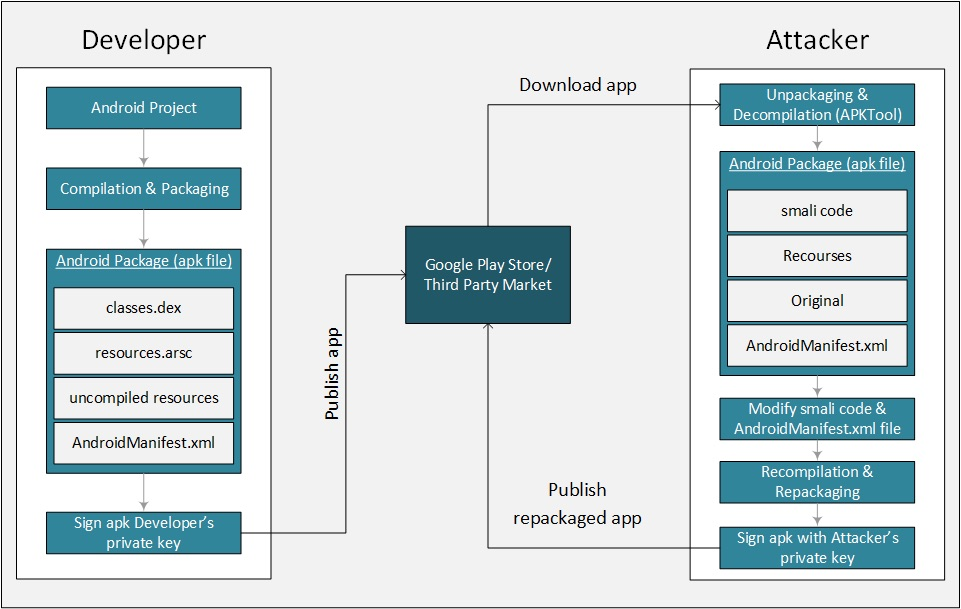
\includegraphics[scale = 0.50]{./imgs/repackAttack}
	\end{figure}
	
	
	\indent
	In order to overcome the above mentioned attack there have been developed Android Packers that can enhance Android applications by providing anti-decompliation, anti-runtime injection and anti-debug techniques. The Android Packers are available only through  where the developer can upload his apk file and get it in \textit{packed} form which is safer for distribution on application markets.  However, recently the Android Packers have started to be used not only by developers to protect their intelectual property but also by hackers to better hide malware in applications (Yang et al, 2015).  A packed application  poses a real challenge for cybersecurity specialists because it is really hard to be analyzed to detect if is bening or malicious.  


\section{Literature review}(10p - 1000w)\\

\subsection{DroidUnpack}
	DroidUnpack is a framework developed for detection and analysis of Android applications with packed malware and it can monitor app execution at the lowest level and also reconstruct Java level execution (Duan et al., 2018). In other words, DroidUnpack is an emulator that can run the Android OS with the app to be analysed and monitors the memory writes performed by the application. The framework has been tested against 93 910 Android applications containing malware (13 556 containing packed malware), 6 major commercial packers (Ali, Baidu, Bangle, Ijami, Qihoo and Tencent) and 3 unpackers (DexHunter, AppSpear and Kisskiss) over a large time frame (2010 - 2015) and the authors want to make it public in the future.\\
	DroidUnpack makes use of the following tools to investigate a packed application:

	\begin{enumerate}
		\item  JNI inspector
		\item  Hidden Code Extractor
		\item  Multi-layer Unpacking Detector
		\item  Self-Modifying Code Detector
	\end{enumerate}

   	\indent
	When developing an Android application the developer can use multiple languages like Java, C++ and C. The \textbf{J}ava \textbf{N}ative \textbf{I}nterface (JNI) is a framework that enables communication between code written in Java and code written in C/C++ (which is put in libraries referred to as \textit{native libraries}). Attackers can avoid static analysis detection of Android API sensitive calls by creating recursive calls between methods written in C++ and methods written in Java thus JNI inspector tool tries to track the whole sequence of method calls.\\
	\indent
	The Hidden Code Extractor feature extracts hidden packed executable at runtime by making use of the \textit{program counter} (pc) and interceptions of every memory write.\\
	\indent
	Once an executable is launched it is possible to modify it's code and this is known as \textit{self-modifying code}. For example, on Android one can call native code using JNI that in turn can access memory locations storing DEX bytecode and modify them. Moreover, using the same procedure even data structures used by DEX bytecode can be modified in memory, thus self-modifying code is indeed a powerful practice. The Self-Modifying Code Detector tool finds self-modifying code by searching for \textit{execute - write - execute} on the same memory location.\\
	\indent
	The Multi-Layer Unpacking tool looks for code that is continuously decrypted but not executed and only when the execution takes place it is considered the end of a layer, this tool also inspects the memory writes.\\
	\indent
	If an application requires multiple processes to be run (very unlikely for a benign app) the framework can detect when a \textit{fork} takes place and can link a new process to the parent process from which it was created. This behaviour is achieved by modifying the \textit{libcutils.so} native library and is very useful in order to understand what an app does under the hood.\\
	\indent
	DroidUnpack supports only Android 4.2 and 5.0 at the moment which is an drawback in my opinion considering that the current version of Android is 9.0 and there are not that many devices on the market that still run Android 4.2/5.0 . However, the authors of the framework say that DroidUnpack can be easily tweaked to support other Android versions. Another shortcoming of DroidUnpack is the fact that it cannot analyze applications that have anti-emulation detection (i.e. the apps detect that they are running on an emulator and modify their behaviour). The problem with apps that have anti-emulation in place is faced by the vetting process of Google Store as well.  Google also runs the apps on an emulator for a specific time amount (e.g. 24h) to analyse their behaviour  but an attacker could code the app to launch  an attack only after the app has been used for more than one week let us say. 
	For a general view of the DroidUnpack framework please see Figure~\ref{droid} (Duan et al., 2018).


	\begin{figure}[H]
		\centering
		\caption{Overview of the DroidUnpack framework}
		\label{droid}

		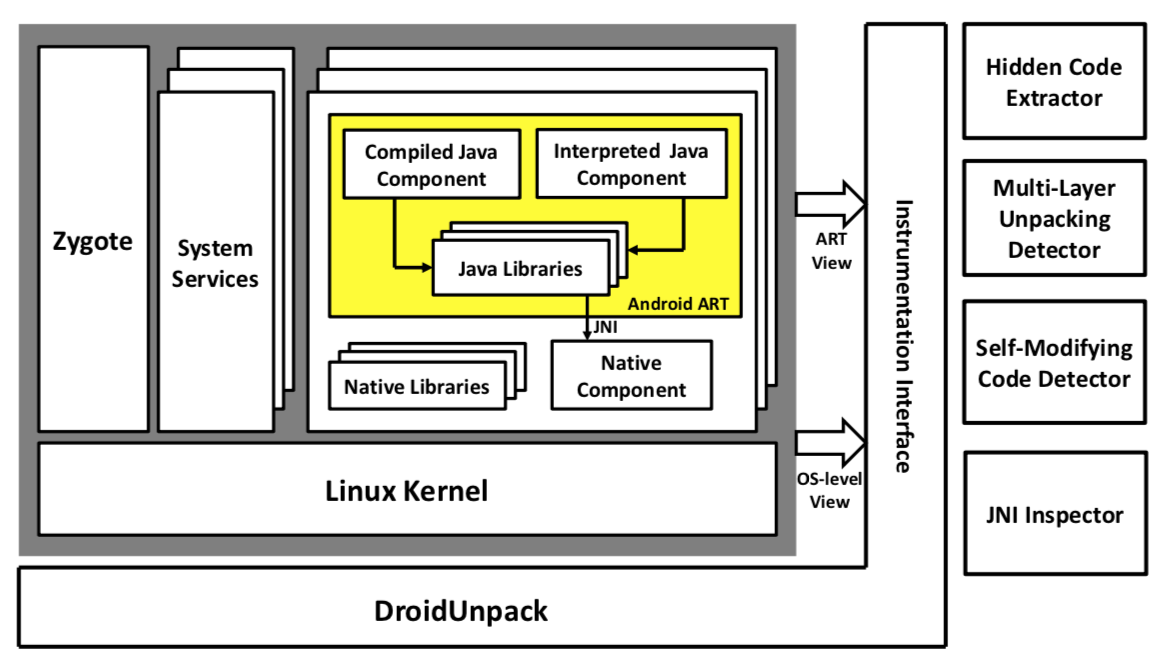
\includegraphics[scale = 0.8]{./imgs/droidUnpack}
	\end{figure}
	
\subsection{DexHunter}
	One important step in finding if a packed app contains  malware is to do a static analysis on the source code of the app. However, a packed application has anti-decompilation protection so it is not easy to get to the DEX code. DexHunter is a software system that can extract the DEX files of a packed application, also known as unpacker software (Zhang, Luo and Yin, 2015). Starting with Android 4.4 the runtime \textbf{D}alvik \textbf{V}irtual \textbf{M}achine (DVM) was replaced with \textbf{A}ndroid \textbf{R}un\textbf{t}ime (ART), nonetheless, DroidHunter works with both runtimes. The unpacker was tested on applications that were packed with six major packers (Bangle, Tencent, 360 Mobile, Ijiami, Ali and Baidu).\\
	\indent
	In order to get to the unpacked DEX bytecode DexHunter works on a physical device when the app to be analysed is running and locates the memory region that the app uses and dumps it. Two approaches have been devised for the two different Android runtimes, DVM and ART. However, in order to obtain the DEX bytecode the authors of DexHunter have modified the DVM and ART runtime on the physical phones where DexHunter was run. Every packer introduces some kind of overhead to the packed application, it could be extra files, new classes or a modified \textit{AndroidManifest.xml}. The authors of DexHunter profiled what files each studied packer introduces so that DexHunter can determine with which packer an app was packed. For applications that are potentially packed with unknown packers (not the 6 ones mentioned above) DexHunter looks for dynamic code modification and if that happens it regards an app as being packed.
	In the Figure~\ref{dexHunt} (Zhang, Luo and Yin, 2015) it can be seen an overview of the whole process that DexHunter uses to get the DEX files of a packed app.

	\begin{figure}[H]
		\centering
		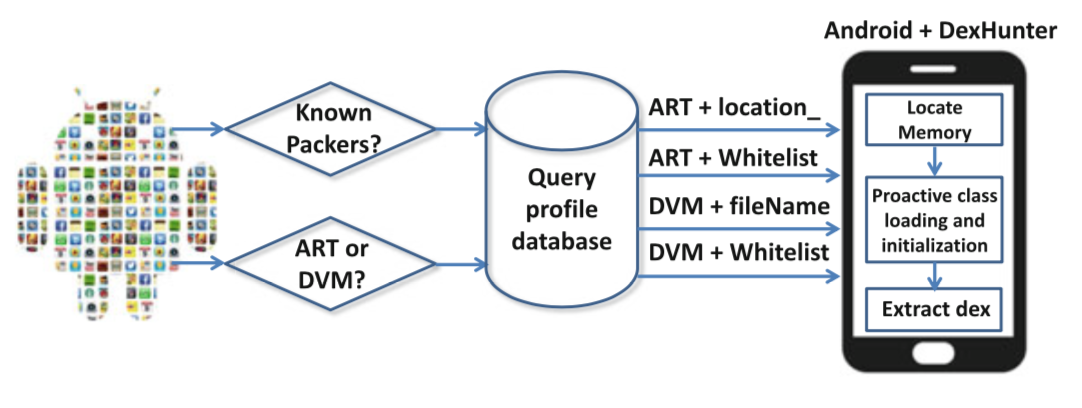
\includegraphics[scale = 0.8]{./imgs/dexHunterFlow}
		\caption{Using DexHunter in smartphone to recover DEX files from packed apps}
		\label{dexHunt}
	\end{figure}

	The evaluation of the DexHunter was done by running it against 40 applications downloaded from F-Droid market which were packed by the authors using the 6 packers mentioned above. However, not all 40  applications could be packed and some of them were not running after being packed. It was found that the packed apps are in general larger and have a prolonged launch time than the original ones. DexHunter managed to recover the DEX files for apps packed with Ijiami, 360 Mobile, Baidu and Bangle packer in both ART and DVM; for Bangle the dumped DEX files were incomplete. Ali packer only works packs apps for DVM runtime and DexHunter managed to get the DEX files for apps packed with Ali packer. 

\newpage

\section{Security and privacy advancement and glitches} (10p - 1000w)
	In the following lines the authors is going to summarise the effects of packed app malware.

\myparagraph{Advertisment}
	\indent
	One of the main incentives for cloning an application is for material gain, thus, an attacker normally picks applications that are popular on Google Store and gets their apk (Gibler et al., 2013). Each published application contains a developer id which is used to direct advertisment revenue to the developer and can be changed. The attacker changes the developer id to himself, repackages the app and publishes it on another market and the advertisment revenue goes to the attacker. Another way of redirecting the advertisment revenue is to change the advertisment libraries used by the app.

\myparagraph{API key}
	\indent
	Most of the cloud services available to Android applications use a key to identify the traffic generated by an app and charge the developer accordingly. Often beginner developers or developers who are not aware that their app can be reverse engineered just store their API keys as constants in app source code. It is obvious that once the API key gets in to the hands of the attacker he can use it in his own applications without being charged for the used services. It is very hard for the developers to find out that their API key is compromised.

\myparagraph{App cracking}
	\indent
	One way to generate revenue is to provide a limted access to some of the app features and for others the developer can require the user to pay to get a 'pro' version. Once the app is decompiled the attacker can identify where the check to see if the user has payed for the pro variant is done, take it out, repackage the app and distribute it on third-party markets. 

\myparagraph{Credential sniffing}
	\indent
	In order to provide personal content to a user many applications use an login mechanism. Once the application is decompiled the attacker can interfere with the authentification mechanism and steal the login credentials of the users.

\myparagraph{Financial fraud}
\indent
	Many Android games today are played by the young generation and due to their competitive nature some of them provide different in-app purchases to enhance the gameplay experience. A repackaged application can circumvent the need for payment for in-app purchases thus it will lure users to download and use it. Once the application is downloaded the attacker can ask for additional permissions non-related to the app and steal sensitive information (Ruiz, 2016). Another possibility is to direct the revenue for the in-app purchases from the developer to the attacker.

\myparagraph{Man-in-the middle attacks}
\indent

\section{Real-world scenarios, use cases}(8p - 800w)\\
%examples to demonstrate the impact
%talk about DroidDream Trojan
%Zeus
%SMSSend
%talk about Obfuscated Malware discovered on google Play
\section{Conclusion}(5p - 500w)\\


\pagebreak
\section{References}

Crussell, J., Gibler, C. and Chen, H. (2012) \underline{Attack of the clones: Detecting cloned}\\ \underline{applications on android markets} In European Symposium on Research in Computer Security  Berlin : Springer\\


Duan, Y., Zhang, M., Bhaskar, A.V., Yin, H., Pan, X., Li, T., Wang, X. and Wang, X. (2018) \underline{Things you may not know about android (un) packers: a systematic study}\\ \underline{ based on whole-system emulation} In 25th Annual Network and Distributed System Security Symposium  s.l. : NDSS \\

\underline{F-Droid} (n.d.) [Online] Available: https://f-droid.org/en/ [Accessed: 26 March 2019]

Gibler, C., Stevens, R., Crussell, J., Chen, H., Zang, H. and Choi, H. (2013) \underline{Adrob: }\\ \underline{Examining the landscape and impact of android application plagiarism} In Proceeding of the 11th annual international conference on Mobile systems, applications, and services s.l : ACM\\

\underline{Google I/O 2017.} (n.d.) [Online] Available: https://bit.ly/2CvBOjd [Accessed: 12 March 2019].\\

\underline{Mobile OS Market Share 2018.} (2019) [Online] Available: https://bit.ly/2Fwii8f [Accessed: 24 March 2019].\\

Ruiz, F. (2016) \underline{Obfuscated Malware Discovered On Google Play} [Online]  Available: https://bit.ly/2UcWx5y [Accessed: 12 March 2019] \\

Shao, Y., Luo, X., Qian, C., Zhu, P. and Zhang, L. (2014) \underline{Towards a scalable}\\ \underline{resource-driven approach for detecting repackaged Android applications} In Proceedings of the 30th Annual Computer Security Applications Conference  s.l: ACM\\

Tumbleson, C. (n.d.) \underline{Apktool.} [Online] Available: https://ibotpeaches.github.io/Apktool/ [Accessed: 24 March 2019].\\

Wenliang, D. (2015) \underline{Android Repackaging Attack Lab} [Online]\\ Available: https://bit.ly/2urlfRa  [Accessed: 24 March 2019]\\

Yang, W., Zhang, Y., Li, J., Shu, J., Li, B., Hu, W. and Gu, D. (2015)\\ \underline{Appspear: Bytecode decrypting and dex reassembling for packed android malware}. In International Workshop on Recent Advances in Intrusion Detection (pp. 359-381) Cham: Springer \\

Zhang, Y., Luo, X. and Yin, H., (2015)  \underline{Dexhunter: toward extracting hidden code}\\ \underline{from packed android applications}  European Symposium on Research in Computer Security (pp. 293-311) Cham: Springer\\

\end{document}

